\chapter{SYSTEM ARCHITECTURE AND METHODOLOGY}

\section{Block Diagram}

The process of converting a handwritten circuit diagram into a structured netlist involves a series of coordinated steps, each step feeding into the next, designed to detect, extract, and represent pictorial information in a machine-readable format and then using this data for simulation and schematic generation.

\begin{figure}[H]
    \centering
    
\includegraphics[width=\textwidth]{src/images/figures/block_diagram.png}
    \caption{Block Diagram of the CIRCUITRON System}
    \label{fig:block-diagram-circuitron}
\end{figure}

The high-level architecture of the CIRCUITRON system is visualized in the block diagram in Figure~\ref{fig:block-diagram-circuitron}. Each step involved in the hand-drawn image to simulation-ready schematic pipeline is elaborated as follows.

\subsection{Preprocessing}

At first, the circuit information (components, component values, units, wire intersection, etc.) needs to be extracted out from the hand-drawn image. Appropriately fine-tuned ML and DL models are to be used for each of these steps which will be elaborated on in later subsections, however, for any sort of detection to happen, the image needs to first be pre-processed. Preprocessing for this not only includes image manipulation tasks but also conversion of the dataset annotations into appropriate formats to maintain compatibility with the component detection and text recognition models. The dataset of choice is in the Pascal VOC format which is incompatible with the models that are intended to be used in the pipeline and hence need to be converted. The code for this conversion with examples will be discussed in the implementation section.

Furthermore, image preprocessing, which includes steps like denoising, contrast and brightness enhancement (for improved clarity) is a vital step in readying the dataset for training any and all models. However, geometric augmentations, especially rotation, is not appropriate for this project.

Among the various available preprocessing techniques, the ones to use are to be selected with careful consideration of the type of images available in the dataset as well as the models in use. Besides image manipulation using various techniques, preprocessing also includes splitting the dataset into training, validation and testing subsets as appropriate.

\subsection{Circuit Component Detection}

A critical step in the pipeline is the accurate detection of circuit components from hand-drawn schematic images. This task is addressed using a real-time object detection algorithm capable of identifying and localizing multiple electronic components (like resistors, capacitors, voltage sources, etc.) directly within the image. YOLO algorithm, the YOLOv7 model, specifically, has been selected for the component detection needs of this project. It is to be noted that text, as a generic collection of letters, numbers, and special characters is also considered a component in this context.

\gls{yolo} (You Only Look Once) is a real-time object detection algorithm known for speed and efficiency. YOLO frames object detection as a single regression problem, straight from image pixels to bounding box coordinates and class probabilities. This model works as follows: first, dividing the image into an $S \times S$ grid. Each grid cell is responsible for detecting objects whose centre falls within it. For each cell, a number of bounding boxes and their corresponding confidence scores (which represents the accuracy of the box and whether the box contains an object) are predicted. Each predicted bounding box includes the coordinates of the box centre relative to grid cell, represented by $(x,y)$, the width and height relative to the whole image, represented by $(w,h)$ and the confidence score $C$ given as:

\begin{equation}
C = P(\text{object}) \cdot \text{IoU}
\label{eq:yolo-confidence-score}
\end{equation}

where $P(\text{object})$ denotes the probability of an object being inside the box, and \gls{iou} is the Intersection over Union between the predicted box and the ground truth box.

Additionally, for each box, class probabilities are predicted as:

\begin{equation}
\text{Class Score} = P(\text{class } i \mid \text{object}) \cdot C
\label{eq:yolo-class-score}
\end{equation}

This allows the model to classify which object exists in each box and once the predictions are made, non-maximum suppression (\gls{nms}) is applied to discard less-relevant overlapping boxes.

Based on similar fundamental working principle, several iterations (versions) of YOLO have been introduced and popularized among which YOLOv7 is the YOLO model of choice for this project.

\begin{figure}[H]
    \centering
    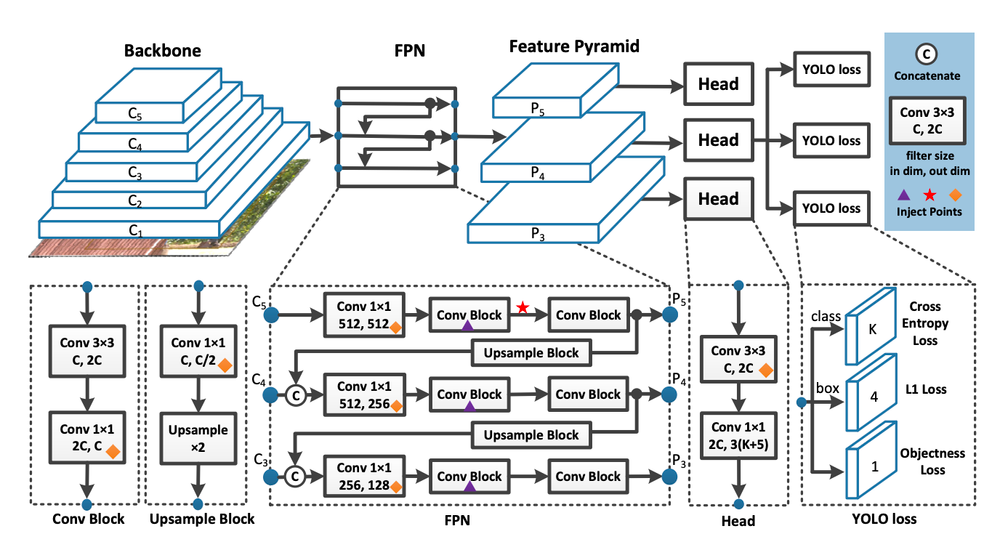
\includegraphics[width=\textwidth]{src/images/figures/yolov7_architecture.png}
    \caption{Architecture of YOLOv7}
    \label{fig:yolov7-architecture}
\end{figure}

The architecture of the YOLOv7 model is composed of three primary modules: Backbone, Neck, and Head.

\begin{itemize}
    \item \textbf{Backbone:} YOLOv7 uses an extended version of \gls{elan} (Efficient Layer Aggregation Network) as its backbone. This structure enables deeper network designs without significantly increasing computational cost. The backbone is responsible for extracting hierarchical features from the input image while preserving gradient flow and feature reuse.
    
    \item \textbf{Neck:} The neck in YOLOv7 incorporates a Path Aggregation Network (\gls{pan}) and ELAN-W modules. PAN enhances feature fusion across different scales, improving detection accuracy for both small and large objects. ELAN-W further refines spatial and contextual information during feature aggregation.
    
    \item \textbf{Head:} The head predicts object classes, bounding box coordinates $(x,y,h,w)$, and objectness scores. YOLOv7 uses a decoupled head, which separates classification and regression branches for better convergence and performance. The model outputs predictions at multiple scales to capture objects of varying sizes.
\end{itemize}

Further features of the model are as follows:

\begin{itemize}
    \item \textbf{Bounding Box Prediction:} The prediction of bounding box coordinates in YOLOv7 is guided by anchor-based regression, where the final bounding box $B=(x,y,w,h)$ is computed relative to the anchor box using the following formula:
    
    \begin{equation}
    x = \sigma(t_x) + c_x
    \label{eq:bbox-x}
    \end{equation}
    
    \begin{equation}
    y = \sigma(t_y) + c_y
    \label{eq:bbox-y}
    \end{equation}
    
    \begin{equation}
    w = p_w \cdot e^{t_w}
    \label{eq:bbox-w}
    \end{equation}
    
    \begin{equation}
    h = p_h \cdot e^{t_h}
    \label{eq:bbox-h}
    \end{equation}
    
    where $(t_x, t_y, t_w, t_h)$ are the predicted offsets, $(c_x, c_y)$ is the top-left corner of the grid cell, and $(p_w, p_h)$ are the dimensions of the anchor box.
    
    \item \textbf{Training Enhancements:} YOLOv7 introduces Coarse-to-Fine Lead Head, Model Scaling, and Auxiliary Heads that help improve gradient flow and stability during training. It supports Label Assignment Strategies such as dynamic-k matching for optimal anchor-label association.
    
    \item \textbf{Data Augmentation:} YOLOv7 applies automatic data augmentation during training including mosaic augmentation (combining four images into one), \gls{hsv} color augmentation, and random flipping, cropping, and scaling. These help increase dataset diversity and improve generalization.
    
    \item \textbf{Early Stopping and Training Stability:} YOLOv7 supports built-in early stopping based on a patience threshold if validation loss (combining box loss, objectness loss, and classification loss) does not improve for several epochs. This ensures faster convergence and prevents overfitting.
\end{itemize}

\subsection{Recognition of Component Values}

In order to generate a complete and simulation-ready netlist, it is essential to not only detect the components themselves but also to extract their associated parameter values, which are generally annotated near the components in the circuit diagram. Thus, it becomes essential to integrate Optical Character Recognition (\gls{ocr}) with the object detection pipeline to extract and map these values correctly to the corresponding components.

This involves identifying regions within the circuit image that likely contain text (done by YOLOv7), and then recognizing said texts in order to parse the component values along with their units.

The hand-written text recognition is done using a \gls{crnn}-based \gls{ocr} system, following the design philosophy of Deep Text Recognition Benchmark (DTRB) framework, however minor changes deemed suitable for this project have been made to get the text detection and recognition pipeline.

\begin{figure}[H]
    \centering
    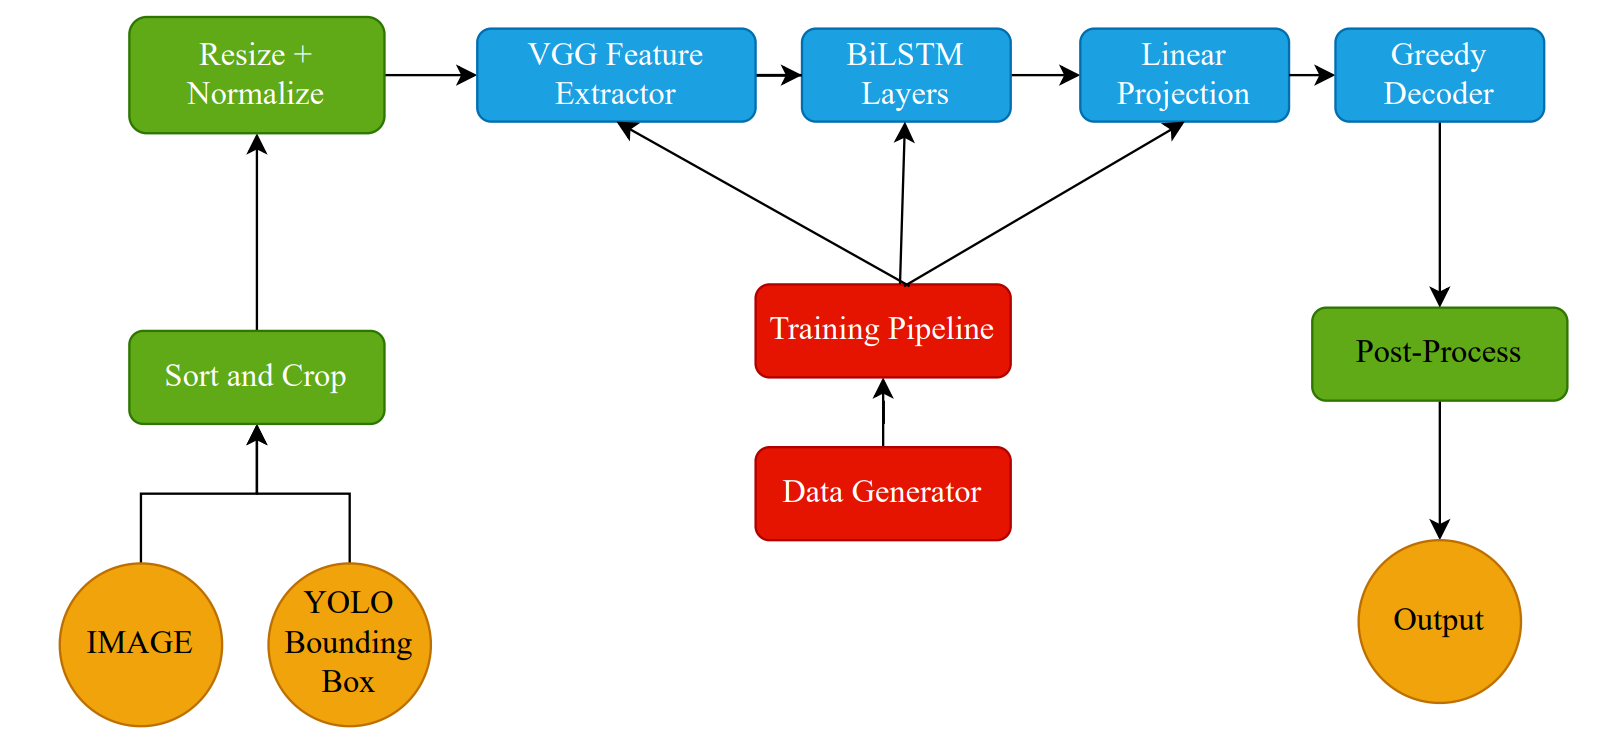
\includegraphics[width=\textwidth]{src/images/figures/easyocr_architecture.png}
    \caption{Text Detection and Recognition Pipeline}
    \label{fig:text-recognition-pipeline}
\end{figure}

YOLOv7 outputs (bounding box information) help segregate textual information (class `0' in the used dataset) which are then cropped, resized (to image height as 32) and normalized for compatibility with text recognition module. This is then passed through to a \gls{crnn} architecture composed of a Convolutional Encoder, Sequence Modeling Engine with Linear Projection, and \gls{ctc} Decoder.

\textbf{Convolutional Encoder (CNN):} A \gls{cnn} stack (e.g., VGG) transforms input image $I$ from multi-dimensional $\mathbb{R}^{H \times W \times C}$ to feature maps:

\begin{equation}
F = f_{\text{CNN}}(I_i), \quad F \in \mathbb{R}^{H' \times W' \times C}
\label{eq:cnn-encoder}
\end{equation}

\textbf{Sequence Modeling (Bidirectional LSTM):} Each $F$ becomes input to a bidirectional \gls{lstm}, yielding hidden states $h_t$. These hidden states capture context across the text line, allowing modeling of character sequences:

\begin{equation}
\overrightarrow{h_t} = \text{LSTM}_f(F_t, \overrightarrow{h_{t-1}})
\label{eq:bilstm}
\end{equation}

\textbf{CTC Decoder:} A softmax layer projects $h_t$ over the character vocabulary as:

\begin{equation}
p_{t,k} = \frac{e^{W_k h_t + b_k}}{\sum_{k'} e^{W_{k'} h_t + b_{k'}}}
\label{eq:ctc-softmax}
\end{equation}

The probability of sequence $z$ is computed over all alignments:

\begin{equation}
P(z \mid y) = \sum_{\pi: B(\pi)=z} \prod_{t=1}^{T} p_{t,\pi_t}
\label{eq:ctc-probability}
\end{equation}

The \gls{ctc} loss is given by the negative logarithm of $P(z \mid y)$. It enables end-to-end sequence decoding without explicit character bounding boxes.

During inference, greedy decoding strategy is used which selects the most-probable character at each time step while removing blank symbols and collapsing consecutive duplicate characters. The recognized text then needs to be mapped to the appropriate circuit component whose value it represents.

\subsection{Wire Detection}

Wire detection is performed using junction points detected by the object detection model as structural anchors for circuit connectivity. All detected junctions are first transformed from normalized detection space to pixel coordinates to ensure geometric consistency within the image domain. Pairwise combinations of junction points are then analyzed to identify potential wire candidates.

For each junction pair, a displacement vector and its orientation angle are computed. Based on a predefined angular tolerance, only near horizontal and near vertical orientations are retained, while diagonal connections are rejected to conform with standard schematic drawing conventions. Valid pairs are projected onto strict axis-aligned representations to form candidate wire segments.

To improve robustness against detection noise, wire endpoints are snapped to a uniform grid and collinear segments are consolidated using proximity and overlap criteria. This produces a compact and topologically consistent set of horizontal and vertical wire segments that represent the underlying circuit wiring.

\subsection{Terminal Point Detection}

Terminal point detection focuses on identifying meaningful electrical connection points associated with wires and components. Junction detections from the object detection model serve as primary terminal candidates, representing wire endpoints, intersections, and branching locations.

Once the final wire set is established, terminal points are refined by analyzing intersections between axis-aligned wire segments and component bounding boxes. Each intersection corresponds to a valid electrical terminal where a wire connects to a component edge. Intersection conditions are evaluated analytically to ensure precise localization of entry and exit points.

The resulting terminal points form a complete connectivity interface between wires and components, enabling accurate circuit graph construction and frontend mapping. This structured representation supports subsequent tasks such as netlist generation, interactive visualization, and automated circuit understanding.

\subsection{Integration Algorithm}

From the individual outputs from each of the aforementioned modules, the task is now to generate a structured \gls{json} representation of the circuit which will be used to generate a corresponding \gls{spice} netlist and also contribute in the schematic generation further down the line.

The integration between all these different outputs, in a simplistic form, would consist of the following steps:

\begin{itemize}
    \item Get a list of components and their corresponding bounding box coordinates (from YOLOv7).
    
    \item Get a list of text data and their corresponding bounding box coordinates (from \gls{ocr}).
    
    \item Map the component to the corresponding component value (text) based on the minimum Euclidean distance between a particular component and texts on the circuit.
    
    \item Once the terminals are determined based on the bounding boxes, match those terminal points to the nearest nodes in the circuit.
    
    \item Store the accumulated information in a \gls{json} file.
\end{itemize}

\subsection{SPICE Netlist Generation}

A netlist is a file that describes the connections between components in an electronic circuit. It acts as a blueprint, specifying which components are connected and how, without detailing the physical layout or specific component placement.

A \gls{spice} netlist is a text-based representation of an electrical circuit used for simulation by a \gls{spice} engine. It provides all the necessary information about the components, their connections, and their electrical properties, enabling analysis such as transient response, DC/AC sweep, or frequency domain behavior.

The netlist serves as input to a circuit simulation engine (NgSpice), which then performs numerical computations to evaluate how the circuit behaves under specified conditions.

For each component, the \gls{spice} netlist contains the information about its name, the nodes it is connected to on either side and the component's parameters or model (if necessary) in the following format:

\begin{center}
\texttt{<Component\_Name> <Node1> <Node2> <Value>}
\end{center}

After the \gls{json} file with abundant information about the components, their values, and the nodes they are connected to is generated, the next step is to convert said \gls{json} file into a netlist format (a \texttt{.txt} file which follows the appropriate conventions).

\subsection{Digital Schematic Generation}

The \gls{json} file built by integrating all the information about the hand-drawn circuit is to be manipulated through different JavaScript libraries to generate a digital, editable schematic of the circuit. As briefly discussed in the Requirements section, Chart.js is to be used to map each component in \gls{json} to a visual block (a symbol for the component as given by the KiCad symbol library). For each component, a graphical symbol needs to be rendered at a certain position and connection lines need to be drawn between the terminals and node positions. A rough pseudocode for the same is as follows:

\begin{algorithm}
\caption{Frontend Circuit Rendering}
\label{algo:frontend-rendering}
\begin{algorithmic}
\Require Circuit \gls{json} description $J$
\Ensure Rendered circuit schematic
\For{all component $c \in J.\text{components}$}
    \State Draw schematic symbol of type $c.\text{type}$ at position $c.\text{position}$
    \State Attach text label $c.\text{value}$ near component position
\EndFor
\For{all connection $k \in J.\text{connections}$}
    \State Retrieve terminal position from $k.\text{from}$ and terminal index
    \State Retrieve node position from $k.\text{node}$
    \State Draw wire between terminal and node positions
\EndFor
\State \Return Rendered schematic
\end{algorithmic}
\end{algorithm}

In order to make the schematic editable, Chart.js allows for draggable elements using inbuilt functions like \texttt{onDrag}, transformation handles for resizing and rotating, with added functions (and work-arounds in some cases) for integration of editing features like editing component value, delete/add components, etc. Changes can be saved by updating the \gls{json} structure on every interaction.

\subsection{Backend Development}

The backend is to be constructed using Next.js and FastAPI, functioning as the core middleware responsible for routing, processing, and orchestrating the system's \gls{ml} pipeline and user interactions. All endpoints follow a RESTful \gls{api} design, ensuring stateless and scalable communication between the frontend and the server.

Upon receiving a hand-drawn circuit image through an \gls{api} endpoint like \texttt{/upload}, the image is saved to a temporary storage location. The server invokes the YOLOv7 model (via a Python subprocess or containerized inference \gls{api}) to detect and localize electrical components. Simultaneously, the \gls{ocr} model is invoked to extract nearby textual annotations. The result is a list of components with bounding boxes and a list of recognized texts, each with confidence scores and coordinates.

Support for user interaction with the schematic is also handled by the backend. Operations such as component deletion, repositioning, wire addition, and modification of values are processed through specific \gls{api} endpoints. Each update is stored in the database, maintaining a real-time editable circuit representation. This allows the frontend to continuously reflect changes without direct manipulation of the database, ensuring security and stability of the system.

\subsection{LLM Integration}

To enhance interaction with the circuit beyond \gls{gui} manipulation, a large language model (\gls{llm}) is to be integrated, facilitated through LangChain and LangGraph. LangChain constructs the agent architecture responsible for handling user queries, such as, ``Explain the purpose of this resistor.'', ``Identify possible errors in this circuit.'', etc. The agent receives contextual data from the backend (such as the circuit's \gls{json} structure or \gls{spice} netlist), formats the prompt, and forwards it to the \gls{llm} through a secure \gls{api}. LangGraph manages the session state, context memory, and branching logic for multi-turn conversations. This enables the system to remember previously discussed components or simulation outputs across queries.

\section{Wire Detection Methodology}

The detection of wires in circuit diagrams requires a systematic approach that leverages geometric constraints inherent to electrical schematics. This section presents a comprehensive methodology for wire detection and terminal point analysis based on junction points detected by the YOLOv7 object detection framework. The fundamental assumption underlying this work is that circuit wires are predominantly axis-aligned, meaning they run either horizontally or vertically with respect to the image coordinate system.

The image domain is defined as the discrete set $\Omega = \{(x,y) \in \mathbb{Z} : 0 \le x < W, 0 \le y < H\}$ where $W$ and $H$ represent the image width and height in pixels respectively. The \gls{yolo} detection framework operates in a normalized coordinate space $\mathcal{U} = [0,1]^2$, necessitating a transformation to pixel coordinates for subsequent geometric analysis.

\subsection{Coordinate Denormalization}

The \gls{yolo} object detection framework produces detection tuples in normalized form. Each detection is represented as a quintuple $d = (c, x_n, y_n, w_n, h_n)$ where $c \in \mathbb{N}$ denotes the class label, $(x_n, y_n) \in [0,1]^2$ represents the normalized bounding box center, and $(w_n, h_n)$ specifies the normalized dimensions. For wire detection, only junction points are relevant, identified by class label $c = 1$.

The denormalization operator transforms normalized coordinates to pixel space through the affine map $\mathcal{N}^{-1} : \mathcal{U} \to \mathbb{R}^2$ defined as:

\begin{equation}
\mathcal{N}^{-1}(x_n, y_n) = \begin{pmatrix} W \cdot x_n \\ H \cdot y_n \end{pmatrix}
\label{eq:denormalization}
\end{equation}

This transformation constitutes a diagonal linear map with matrix representation $\text{diag}(W, H)$. The operator is bijective with determinant $WH \neq 0$, admitting the inverse $\mathcal{N}(x, y) = (x/W, y/H)$. The pixel-space junction set is thus constructed as $J = \{\mathbf{j} = \mathcal{N}^{-1}(x_n^{(d)}, y_n^{(d)}) : d \in \mathcal{J}\}$ where $\mathcal{J}$ denotes the subset of detections with class label unity.

\subsection{Pairwise Junction Analysis}

The wire detection algorithm operates by examining all possible pairs of junction points. For a junction set of cardinality $n = |J|$, the number of distinct unordered pairs requiring analysis is $\binom{n}{2} = n(n-1)/2$. Each pair $(\mathbf{j}_i, \mathbf{j}_k)$ with $i < k$ generates a displacement vector:

\begin{equation}
\mathbf{d}^{\leftrightarrow} = \mathbf{j}_k - \mathbf{j}_i = \begin{pmatrix} \Delta x \\ \Delta y \end{pmatrix}
\label{eq:displacement-vector}
\end{equation}

where $\Delta x = j_{k,x} - j_{i,x}$ and $\Delta y = j_{k,y} - j_{i,y}$ represent the horizontal and vertical displacements respectively. The magnitude of this displacement vector, given by $\|\mathbf{d}^{\leftrightarrow}\| = \sqrt{\Delta x^2 + \Delta y^2}$, represents the Euclidean distance between the junction pair.

\subsection{Angular Orientation Computation}

The orientation of the displacement vector is computed using the four-quadrant arctangent function, which correctly resolves the angle in all quadrants of the Cartesian plane. The signed orientation angle $\theta \in (-\pi, \pi]$ is defined as:

\begin{equation}
\theta = \text{atan2}(\Delta y, \Delta x)
\label{eq:angular-orientation}
\end{equation}

The \texttt{atan2} function is defined piecewise to handle all possible combinations of signs for its arguments. When $\Delta x > 0$, the angle equals $\arctan(\Delta y / \Delta x)$. When $\Delta x < 0$ and $\Delta y \ge 0$, a correction of $+\pi$ is applied. When $\Delta x < 0$ and $\Delta y < 0$, a correction of $-\pi$ is applied. The degenerate cases where $\Delta x = 0$ yield $\pm\pi/2$ depending on the sign of $\Delta y$.

For classification purposes, the angle is converted to a positive representation in degrees using the transformation $\tilde{\theta} = (180\theta / \pi) \mod 360$, yielding values in the range $[0^\circ, 360^\circ)$.

\subsection{Horizontal and Vertical Line Classification}

The classification of junction pairs as horizontal, vertical, or diagonal is accomplished through angular tolerance zones. The tolerance parameter $\epsilon = 18^\circ$ represents 10\% of the half-circle, providing sufficient margin to accommodate minor deviations from perfect alignment while maintaining classification accuracy.

\textbf{Horizontal Acceptance Region:} The set of angles classified as horizontal is defined as the union:

\begin{equation}
\Theta_H = [0^\circ, 18^\circ] \cup [162^\circ, 198^\circ] \cup [342^\circ, 360^\circ]
\label{eq:horizontal-region}
\end{equation}

This region captures angles within $\pm 18^\circ$ of the positive $x$-axis ($0^\circ$ and $360^\circ$) and within $\pm 18^\circ$ of the negative $x$-axis ($180^\circ$).

\textbf{Vertical Acceptance Region:} The set of angles classified as vertical is defined as:

\begin{equation}
\Theta_V = [72^\circ, 108^\circ] \cup [252^\circ, 288^\circ]
\label{eq:vertical-region}
\end{equation}

This region captures angles within $\pm 18^\circ$ of the positive $y$-axis ($90^\circ$) and within $\pm 18^\circ$ of the negative $y$-axis ($270^\circ$).

\textbf{Diagonal Rejection Region:} The complement of the horizontal and vertical regions constitutes the diagonal rejection region:

\begin{equation}
\Theta_D = [0^\circ, 360^\circ) \setminus (\Theta_H \cup \Theta_V)
\label{eq:diagonal-region}
\end{equation}

Junction pairs whose orientation falls within $\Theta_D$ are rejected as they do not represent valid axis-aligned wires.

The classification function $\mathcal{O} : [0^\circ, 360^\circ) \to \{H, V, \varnothing\}$ maps each angle to its corresponding orientation category. The total angular coverage of valid classifications is $(|\Theta_H| + |\Theta_V|)/360^\circ = 144^\circ/360^\circ = 40\%$, indicating that 40\% of angular space is accepted as orthogonal while 60\% is rejected as diagonal.

\subsection{Orthogonal Projection and Axis Alignment}

For junction pairs with valid orthogonal classification, the detected endpoints must be projected onto perfectly axis-aligned lines to ensure strict horizontal or vertical wire representation. This projection compensates for minor deviations from perfect alignment that fall within the tolerance zone.

\textbf{Horizontal Wire Projection:} For a junction pair $(\mathbf{j}_i, \mathbf{j}_k)$ with classification $\mathcal{O}(\tilde{\theta}) = \text{HORIZONTAL}$, the aligned wire is constructed by computing the mean $y$-coordinate:

\begin{equation}
\bar{y} = \frac{j_{i,y} + j_{k,y}}{2}
\label{eq:horizontal-projection}
\end{equation}

The projected wire endpoints are then defined as $\mathbf{s} = (j_{i,x}, \bar{y})$ and $\mathbf{e} = (j_{k,x}, \bar{y})$. Both endpoints share the same $y$-coordinate, ensuring perfect horizontal alignment.

\textbf{Vertical Wire Projection:} For a junction pair with classification $\mathcal{O}(\tilde{\theta}) = \text{VERTICAL}$, the aligned wire is constructed by computing the mean $x$-coordinate:

\begin{equation}
\bar{x} = \frac{j_{i,x} + j_{k,x}}{2}
\label{eq:vertical-projection}
\end{equation}

The projected wire endpoints are $\mathbf{s} = (\bar{x}, j_{i,y})$ and $\mathbf{e} = (\bar{x}, j_{k,y})$. Both endpoints share the same $x$-coordinate, ensuring perfect vertical alignment.

\textbf{Projection Error Bound:} For a junction pair with orientation angle $\tilde{\theta} \in [0^\circ, \epsilon]$ and inter-junction distance $L = \|\mathbf{d}^{\leftrightarrow}\|$, the maximum perpendicular displacement of any endpoint from its original position is bounded by:

\begin{equation}
\delta = \frac{|\Delta y|}{2} \le \frac{L \sin(\epsilon)}{2}
\label{eq:projection-error}
\end{equation}

For the tolerance $\epsilon = 18^\circ$ with $\sin(18^\circ) \approx 0.309$, this yields $\delta \approx 0.155L$. Thus, for a 100-pixel wire, the maximum projection displacement is approximately 15.5 pixels.

\subsection{Grid Quantization}

To ensure coordinate consistency and facilitate subsequent merging operations, all wire endpoints are quantized to a uniform grid. The grid structure is defined by the integer lattice $\mathcal{G} = g\mathbb{Z} \times g\mathbb{Z}$ where $g \in \mathbb{N}^+$ is the grid resolution, set to $g = 16$ pixels in this implementation.

\textbf{Snap Function:} The scalar quantization operator $\text{snap} : \mathbb{R} \to g\mathbb{Z}$ is defined as:

\begin{equation}
\text{snap}(v) = g \cdot \text{round}\left(\frac{v}{g}\right) = g \cdot \left\lfloor \frac{v}{g} + \frac{1}{2} \right\rfloor
\label{eq:snap-function}
\end{equation}

The vectorized extension $\text{Snap} : \mathbb{R}^2 \to \mathcal{G}$ applies the scalar operator component-wise, yielding $\text{Snap}(\mathbf{p}) = (\text{snap}(p_x), \text{snap}(p_y))$.

\textbf{Quantization Error Bounds:} For any scalar value $v \in \mathbb{R}$, the quantization error satisfies $|v - \text{snap}(v)| \le g/2$. For any vector $\mathbf{p} \in \mathbb{R}^2$, the error bounds are:

\begin{equation}
\|\mathbf{p} - \text{Snap}(\mathbf{p})\|_\infty \le \frac{g}{2}, \quad \|\mathbf{p} - \text{Snap}(\mathbf{p})\|_2 \le \frac{g\sqrt{2}}{2}
\label{eq:quantization-error}
\end{equation}

For $g = 16$ pixels, the maximum coordinate error is 8 pixels and the maximum Euclidean error is approximately 11.3 pixels.

\subsection{Wire Segment Consolidation}

The pairwise analysis of junctions frequently generates multiple overlapping wire segments that represent the same physical wire. The consolidation algorithm merges collinear segments within a tolerance threshold to produce a minimal set of non-redundant wires.

\textbf{Canonical Axis-Aligned Representation:} Each wire segment is transformed to a canonical form $\sigma = (a, \ell_{\min}, \ell_{\max}, \omega)$ where $a$ denotes the fixed axis coordinate ($y$-coordinate for horizontal wires, $x$-coordinate for vertical wires), $[\ell_{\min}, \ell_{\max}]$ specifies the extent along the variable axis, and $\omega \in \{H, V\}$ indicates the orientation.

For a horizontal wire $w = (\mathbf{s}, \mathbf{e}, H)$, the canonical form is $\sigma(w) = (s_y, \min(s_x, e_x), \max(s_x, e_x), H)$. For a vertical wire, the transformation is $\sigma(w) = (s_x, \min(s_y, e_y), \max(s_y, e_y), V)$. The segment length is defined as $L(\sigma) = \ell_{\max} - \ell_{\min}$.

\textbf{Mergeability Relation:} Two segments $\sigma_1$ and $\sigma_2$ with identical orientation are mergeable, denoted $\sigma_1 \sim \sigma_2$, if and only if:

\begin{equation}
|a_1 - a_2| \le \tau \land \ell_{\min}(\sigma_2) \le \ell_{\max}(\sigma_1) + \tau
\label{eq:mergeability}
\end{equation}

where $\tau = g$ is the grid tolerance and the segments are ordered such that $\ell_{\min}(\sigma_1) \le \ell_{\min}(\sigma_2)$. The first condition ensures proximity along the fixed axis, while the second condition requires overlap or near-touching along the variable axis.

\textbf{Merge Operator:} For mergeable segments $\sigma_1 \sim \sigma_2$, the merge operation produces a consolidated segment $\sigma_1 \oplus \sigma_2 = (a_{\text{merged}}, \ell_{\text{merged,min}}, \ell_{\text{merged,max}}, \omega)$ where:

\begin{equation}
a_{\text{merged}} = \begin{cases} a_1 & \text{if } L(\sigma_1) > L(\sigma_2) \\ a_2 & \text{otherwise} \end{cases}
\label{eq:merge-axis}
\end{equation}

\begin{equation}
\ell_{\text{merged,min}} = \min(\ell_{\min}(\sigma_1), \ell_{\min}(\sigma_2)), \quad \ell_{\text{merged,max}} = \max(\ell_{\max}(\sigma_1), \ell_{\max}(\sigma_2))
\label{eq:merge-extent}
\end{equation}

The length-weighted axis selection preserves the axis coordinate of the longer segment, which is assumed to be more geometrically accurate. The extent bounds are computed as the union of the individual extents.

\textbf{Merge Monotonicity:} The merge operation is length-non-decreasing, satisfying:

\begin{equation}
L(\sigma_1 \oplus \sigma_2) \ge \max(L(\sigma_1), L(\sigma_2))
\label{eq:merge-monotonicity}
\end{equation}

The proof follows from the observation that $L(\sigma_1 \oplus \sigma_2) = \max(\ell_{\max}(\sigma_1), \ell_{\max}(\sigma_2)) - \min(\ell_{\min}(\sigma_1), \ell_{\min}(\sigma_2))$. In the containment case where one segment contains the other, the merged length equals the longer segment. In the overlapping case, the merged length exceeds both individual lengths.

The consolidation algorithm proceeds by first separating segments by orientation, then sorting each group by axis coordinate and extent minimum. A linear scan merges consecutive mergeable segments, producing the final consolidated wire set.

\section{Terminal Detection}

Terminal detection refers to the identification of connection points between wire segments and circuit components. These intersection points are critical for establishing the circuit topology and enabling subsequent netlist extraction. This section presents the mathematical framework for detecting wire-component intersections based on axis-aligned bounding box geometry.

\subsection{Component Bounding Box Representation}

Circuit components detected by YOLOv7 are represented as axis-aligned bounding boxes (AABBs). For a detection tuple $d = (c, x_n, y_n, w_n, h_n)$ where $c \notin \{0, 1\}$ (excluding text and junction classes), the pixel-space bounding box is defined as:

\begin{equation}
\mathcal{B} = [x_{\min}, x_{\max}] \times [y_{\min}, y_{\max}]
\label{eq:bounding-box}
\end{equation}

The corner coordinates are computed from the normalized detection parameters as:

\begin{equation}
x_{\min} = \left(x_n - \frac{w_n}{2}\right) W, \quad x_{\max} = \left(x_n + \frac{w_n}{2}\right) W
\end{equation}

\begin{equation}
y_{\min} = \left(y_n - \frac{h_n}{2}\right) H, \quad y_{\max} = \left(y_n + \frac{h_n}{2}\right) H
\label{eq:box-corners}
\end{equation}

The boundary of the bounding box $\partial \mathcal{B}$ consists of four edges: the left edge at $x = x_{\min}$, the right edge at $x = x_{\max}$, the top edge at $y = y_{\min}$, and the bottom edge at $y = y_{\max}$.

\subsection{Wire Component Intersection Analysis}

Consolidated wire segments are represented in parametric form for intersection analysis. A horizontal wire with $y$-coordinate $y_w$ and $x$-extent $[x_{\min}, x_{\max}]$ defines the line segment:

\begin{equation}
\mathcal{L}_H = \{(x, y_w) : x \in [x_{\min}, x_{\max}]\}
\label{eq:horizontal-wire}
\end{equation}

Similarly, a vertical wire with $x$-coordinate $x_w$ and $y$-extent $[y_{\min}, y_{\max}]$ defines:

\begin{equation}
\mathcal{L}_V = \{(x_w, y) : y \in [y_{\min}, y_{\max}]\}
\label{eq:vertical-wire}
\end{equation}

\subsection{Horizontal Wire Intersection Conditions}

The intersection of a horizontal wire with a component bounding box can occur at either the left edge or the right edge of the box. The intersection conditions are derived from the geometric constraints of axis-aligned segments.

\textbf{Horizontal Wire–Left Edge Intersection:} The horizontal wire $\mathcal{L}_H$ with parameters $(y_w, x_{\min}, x_{\max})$ intersects the left edge of bounding box $\mathcal{B} = [x_{\min}, x_{\max}] \times [y_{\min}, y_{\max}]$ at point $(x_{\min}, y_w)$ if and only if:

\begin{equation}
\Phi_L(\mathcal{L}_H, \mathcal{B}) = (y_{\min} \le y_w \le y_{\max}) \land (x_{\min} \le x_{\min} \le x_{\max})
\label{eq:horizontal-left-intersection}
\end{equation}

The first condition $(y_{\min} \le y_w \le y_{\max})$ ensures vertical alignment, requiring that the wire's $y$-coordinate falls within the vertical extent of the box. The second condition $(x_{\min} \le x_{\min} \le x_{\max})$ ensures horizontal overlap, requiring that the left edge $x$-coordinate falls within the horizontal extent of the wire.

The proof of necessity follows from the observation that if an intersection exists at $(x_{\min}, y_w)$, then this point must simultaneously lie on the wire (requiring $y = y_w$ and $x \in [x_{\min}, x_{\max}]$) and on the left edge (requiring $x = x_{\min}$ and $y \in [y_{\min}, y_{\max}]$). Sufficiency is established by verifying that when both conditions hold, the point $(x_{\min}, y_w)$ belongs to both the wire segment and the box boundary.

\textbf{Horizontal Wire–Right Edge Intersection:} The horizontal wire $\mathcal{L}_H$ intersects the right edge of $\mathcal{B}$ at point $(x_{\max}, y_w)$ if and only if:

\begin{equation}
\Phi_R(\mathcal{L}_H, \mathcal{B}) = (y_{\min} \le y_w \le y_{\max}) \land (x_{\min} \le x_{\max} \le x_{\max})
\label{eq:horizontal-right-intersection}
\end{equation}

The structure mirrors that of the left edge intersection, with $x_{\max}$ replacing $x_{\min}$ in the horizontal overlap condition.

\subsection{Vertical Wire Intersection Conditions}

The intersection of a vertical wire with a component bounding box can occur at either the top edge or the bottom edge of the box.

\textbf{Vertical Wire–Top Edge Intersection:} The vertical wire $\mathcal{L}_V$ with parameters $(x_w, y_{\min}, y_{\max})$ intersects the top edge of bounding box $\mathcal{B}$ at point $(x_w, y_{\min})$ if and only if:

\begin{equation}
\Phi_T(\mathcal{L}_V, \mathcal{B}) = (x_{\min} \le x_w \le x_{\max}) \land (y_{\min} \le y_{\min} \le y_{\max})
\label{eq:vertical-top-intersection}
\end{equation}

The first condition $(x_{\min} \le x_w \le x_{\max})$ ensures horizontal alignment, requiring that the wire's $x$-coordinate falls within the horizontal extent of the box. The second condition $(y_{\min} \le y_{\min} \le y_{\max})$ ensures vertical overlap, requiring that the top edge $y$-coordinate falls within the vertical extent of the wire.

\textbf{Vertical Wire–Bottom Edge Intersection:} The vertical wire $\mathcal{L}_V$ intersects the bottom edge of $\mathcal{B}$ at point $(x_w, y_{\max})$ if and only if:

\begin{equation}
\Phi_B(\mathcal{L}_V, \mathcal{B}) = (x_{\min} \le x_w \le x_{\max}) \land (y_{\min} \le y_{\max} \le y_{\max})
\label{eq:vertical-bottom-intersection}
\end{equation}

\subsection{Complete Intersection Set Construction}

The intersection set for a single wire-box pair aggregates all valid intersections across the relevant edges.

\textbf{Wire-Box Intersection Set:} For wire $w$ with orientation $\omega$ and bounding box $\mathcal{B}$, the intersection set is defined as:

\begin{equation}
\mathcal{I}(w, \mathcal{B}) = \begin{cases}
\{(x_{\min}, y_w) : \Phi_L\} \cup \{(x_{\max}, y_w) : \Phi_R\} & \text{if } \omega = H \\
\{(x_w, y_{\min}) : \Phi_T\} \cup \{(x_w, y_{\max}) : \Phi_B\} & \text{if } \omega = V
\end{cases}
\label{eq:wire-box-intersection-set}
\end{equation}

\textbf{Intersection Cardinality Bound:} For each wire-box pair, the cardinality of the intersection set is bounded by $|\mathcal{I}(w, \mathcal{B})| \le 2$. This bound reflects the geometric reality that a straight axis-aligned wire can enter a rectangular box through one edge and exit through the opposite edge, yielding at most two intersection points.

The global intersection set aggregates all wire-box intersections across the complete wire set $\mathcal{W}$ and component box set $\mathcal{C}$:

\begin{equation}
\mathcal{I}_{\text{total}} = \bigcup_{w \in \mathcal{W}} \bigcup_{\mathcal{B} \in \mathcal{C}} \mathcal{I}(w, \mathcal{B})
\label{eq:global-intersection-set}
\end{equation}

\subsection{Terminal Point Significance}

The detected intersection points serve as terminal connection points in the circuit topology. Each intersection $(x, y) \in \mathcal{I}_{\text{total}}$ indicates a location where a wire connects to a component, enabling the construction of a circuit graph where components are nodes and wires are edges. This representation facilitates subsequent circuit analysis tasks including netlist generation, connectivity verification, and schematic reconstruction.

\section{Use-Case Diagram}

The use-case diagram in Figure~\ref{fig:use-case-diagram} outlines the CIRCUITRON system's functionality depicting the interactions between users and the system. The primary actor is the user, who can be a student, instructor, or engineer. The system begins with the user uploading a hand-drawn circuit image.

Upon submission, CIRCUITRON automatically preprocesses the image to enhance clarity and prepares it for further analysis. The system then detects components (e.g., resistors, capacitors) using YOLOv7 and identifies wires and nodes through techniques like junction-based wire detection. Simultaneously, it extracts text labels (e.g., component values) using \gls{ocr} and maps them to the corresponding components.

Once the circuit structure is parsed, the system generates an editable schematic, allowing the user to manually correct any errors before proceeding. After validation, the system converts the schematic into a SPICE-compatible netlist and runs a simulation using Ngspice/PySpice. The results, including voltage and current graphs, are displayed to the user. Additionally, the system integrates an AI assistant to answer circuit-related questions, enhancing the learning and troubleshooting experience.

The ``includes'' relationship is used for mandatory sub-tasks like component detection and \gls{ocr}, which must always execute as part of core workflows. The ``extends'' relationship marks optional features like manual corrections or AI Q\&A, which enhance functionality but aren't required for basic operation. The diagram effectively outlines the system's scope, emphasizing its applications (or use-cases).

\begin{figure}[H]
    \centering
     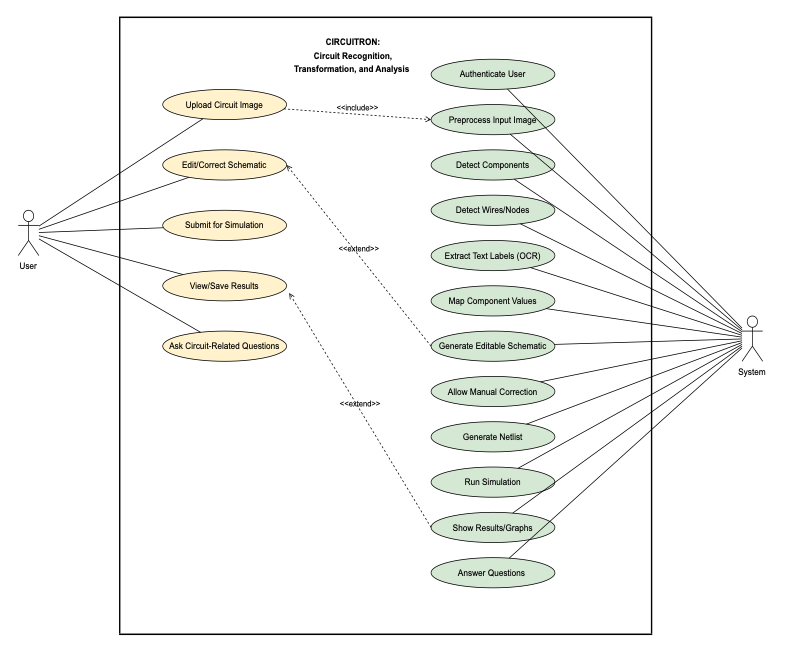
\includegraphics[width=\textwidth]{src/images/figures/use_case_diagram.png}
    \caption{Use-Case Diagram for CIRCUITRON System}
    \label{fig:use-case-diagram}
\end{figure}

\section{Performance Metrics Expectation}

No matter how rigorously the models are trained and fine-tuned, there is always room for error due to edge cases like unclear handwriting and similar-looking components. As such, for any project, it is important to define appropriate performance metrics which indicate when the models can be considered ``good-enough'' for the required purpose. Table~\ref{table:performance-metrics} shows the chosen performance metrics and their target values on achieving which, the training may be stopped.

\begin{table}[H]
    \centering
    \caption{Expected Performance Metric Values for Individual Modules}
    \label{table:performance-metrics}
    \begin{tabular}{lcc}
        \toprule
        \textbf{Pipeline Stage} & \textbf{Performance Metric} & \textbf{Target Value/Expectation} \\
        \midrule
        Component Detection & mAP@0.5 & 0.90 \\
        Text Recognition & Character Accuracy & 0.75 \\
        \bottomrule
    \end{tabular}
\end{table}

\subsection{Component Detection Metric}

mAP@0.5 (mean Average Precision at IoU threshold of 0.5) evaluates how well the model detects components with correct class labels and bounding boxes. It calculates the Average Precision (\gls{ap}) for each class and then takes the mean across all classes. An \gls{iou} (Intersection over Union) threshold of 0.5 means a predicted bounding box is considered a correct match if it overlaps with the ground truth box by at least 50\%.

\begin{equation}
\text{IoU} = \frac{\text{Area of Overlap}}{\text{Area of Union}}
\label{eq:iou-metric}
\end{equation}

A high mAP@0.5 means detections are both precise and complete, minimizing missed or misclassified components.

\subsection{Text Recognition Metric}

Character Accuracy measures how many characters in the predicted text match the actual characters:

\begin{equation}
\text{Character Accuracy} = \frac{\text{Number of Correct Characters}}{\text{Total Number of Characters in Ground Truth}}
\label{eq:character-accuracy}
\end{equation}

In circuit diagrams, values like $10k$, $100\Omega$, $1\mu F$ are crucial. \gls{ocr} must correctly read these values, since even a small error (e.g., mistaking `k' as `1') leads to incorrect simulation behavior. A high character accuracy ensures value-to-component mapping is reliable.

\subsection{Terminal and Node Detection Metrics}

Precision measures how many detected terminals (or nodes) are correct whereas recall measures how many actual terminals (or nodes) were correctly detected:

\begin{equation}
\text{Precision} = \frac{\text{True Positives}}{\text{True Positives} + \text{False Positives}}
\label{eq:precision}
\end{equation}

\begin{equation}
\text{Recall} = \frac{\text{True Positives}}{\text{True Positives} + \text{False Negatives}}
\label{eq:recall}
\end{equation}

Terminals define where components connect to wires, which influences circuit structure. High precision ensures the system doesn't falsely identify noise as terminals, avoiding wrong wire mappings. High recall ensures the system doesn't miss valid terminal points, which would cause incomplete circuits. Likewise, missing nodes can create open circuits, and false nodes can misrepresent actual connectivity. So high values of both precision and recall are crucial for both terminal and node detection.

\section{Error Handling}

In any project with a number of individual modules working together, the overall error not only comes from said individual modules but also from their integration due to propagating errors from one module to another. To handle errors in such a case, foremost the errors in the output of the individual modules need to be controlled and only then can the accumulated error be kept in check. The performance metrics tabulated in the previous section are to be strictly adhered to if there's any hope of generating the \gls{spice} netlist (and digital schematic) with nominal errors.

For the reduction of false matches and \gls{ocr} noise, post-processing techniques such as value format validation, confidence filtering, and text cleanup can be implemented. Value format validation ensures only strings that match known (and appropriate) electrical units, say $10k$, $1\mu F$, $5V$ are retained. Confidence filtering helps discard \gls{ocr} results with low confidence scores, and text cleanup normalizes ambiguous symbols such as converting ``O'' to ``0'', ``$\mu$'' to ``u''.

A basic pseudocode for sample value format validation is as follows:

\begin{algorithm}
\caption{Validation and Filtering of OCR Component Values}
\label{algo:ocr-validation}
\begin{algorithmic}
\Require OCR detected text entries $T$
\Ensure Filtered list of valid component values $V$
\State Define regular expression patterns for resistance, capacitance, and voltage
\State $V \leftarrow \emptyset$
\For{all text entry $t \in T$}
    \If{$t.\text{text}$ matches any defined pattern}
        \State Append $t$ to $V$
    \EndIf
\EndFor
\State \Return $V$
\end{algorithmic}
\end{algorithm}

The list of components shown here is in no way meant to be exhaustive; rather it is to show how this pseudocode ensures that only valid electrical component values are used in the final component-to-value mapping and schematic generation.

To prevent propagating error (error from the output of YOLOv7 bleeding into \gls{ocr}, for instance), a combined confidence threshold checking mechanism can be implemented which marks an item as uncertain if the confidence score from YOLOv7 is less than a certain value (e.g., 0.6) and the same from \gls{ocr} is less than a certain value (e.g., 0.85). For more robustness, a human-in-the-loop mechanism can be implemented which prompts the user to manually approve or correct \gls{ocr}-predicted values, fix connection errors, etc. This can be implemented to trigger when the confidence score is below the set threshold or when other error handling mechanisms such as value format validation fail. The pseudocode for this is as follows:

\begin{algorithm}
\caption{Confidence-Based Error Checking and Validation}
\label{algo:confidence-validation}
\begin{algorithmic}
\Require Module outputs $O$, confidence threshold $\omega$, format validation function $f$
\Ensure Valid outputs $V$ and uncertain outputs $U$
\State $V \leftarrow \emptyset$
\State $U \leftarrow \emptyset$
\For{all item $o \in O$}
    \If{$o.\text{confidence} \ge \omega \land f(o.\text{value})$}
        \State Append $o$ to $V$
    \Else
        \State Append $o$ to $U$
    \EndIf
\EndFor
\If{$U \ne \emptyset$}
    \State Trigger manual override
\EndIf
\State \Return $(V, U)$
\end{algorithmic}
\end{algorithm}

\subsection{Image Augmentation}

Since the dataset contains handwritten circuit diagrams captured under variable lighting and orientations, several augmentation techniques were applied to improve model generalization including Contrast Enhancement (global) and Adaptive Brightness Adjustment by factors of 0.8 and 1.2. Furthermore, geometric augmentation techniques, like spatial flipping (both horizontally and vertically) and rotation (e.g., $90^\circ$ or random rotation) proved to be unwise operations for this project. For example, if a ``C'' is rotated by $90^\circ$, the ``C'' now resembles a ``U'', and the same applies to flipping (``M'' might look like ``W'', for example). Rather than increasing accuracy, it was realized that using rotation or flipping would simply confuse the model. However, continuous testing with other forms of augmentation will continue in hopes of improving the model.

\subsection{Fine-tuning YOLOv5 and YOLOv7 for Component Detection}

YOLOv5 was initially used for benchmarking, and later upgraded to YOLOv7 for better accuracy and inference speed (comparison shown in the Results section). Training and fine-tuning were done using the \gls{cghd} dataset after converting into \gls{yolo}-compatible format.

The training parameters employed are as follows:

\begin{itemize}
    \item \textbf{Number of classes:} 61
    \item \textbf{Training split:} 70\% training, 10\% validation, 20\% testing
    \item \textbf{Epochs:} 200 (for YOLOv5), 100 (for YOLOv7)
    \item \textbf{Image size:} $416 \times 416$ pixels
    \item \textbf{Batch size:} 16 (for YOLOv5), 32 (for YOLOv7)
    \item \textbf{Optimizer:} \gls{sgd} (Stochastic Gradient Descent)
    \item \textbf{Learning rate:} 0.01 (initial)
    \item \textbf{Augmentations used in training:} Mosaic Augmentation, \gls{hsv} Augmentation, Random rotating/flipping
\end{itemize}

\subsection{Implementation of Text Recognition (OCR)}

To extract textual information such as resistor values, capacitor labels, and other component annotations from the circuit diagrams, a \gls{crnn}-based custom \gls{ocr} model was chosen, trained and implemented. The input image in cropped form (cropped for each text component) was passed through this model after training, which returned the content of each detected text element. The position of said text element, however, was found using bounding boxes from YOLOv7. This allowed us to localize and read numerical values or labels directly from the circuit.

Three different modules, each for feature extraction, sequence modeling, and prediction were trained based on the DTRB framework. Initially, simply fine-tuning \gls{ocr} models like TrOCR and EasyOCR were also attempted; however, these didn't yield usable results, ultimately requiring training from scratch. The training was done for 29 epochs.

\subsection{Line Detection Algorithm Implementation}

The line detection mechanism was engineered to exploit the semantic constraints of circuit diagrams, specifically that wires are predominantly axis-aligned (horizontal or vertical) and connect distinct components. Unlike the Probabilistic Hough Transform (\gls{pht}) which operates purely on pixel gradients, this approach uses the junction points detected by YOLOv7 as anchor nodes to reconstruct the wiring layout geometrically.

First, a pairwise analysis was performed on all junction points identified by the object detection model. The algorithm iterates through every unique pair of junctions to calculate the angle of the vector connecting them. Since hand-drawn circuits contain imperfections, an angular tolerance of $\pm 18^\circ$ was applied to classify connections as either horizontal or vertical. To ensure coordinate consistency across the diagram, the resulting segment coordinates were ``snapped'' to a grid using a 16-pixel quantization.

\begin{algorithm}
\caption{Wire Classification and Alignment}
\label{algo:wire-classification}
\begin{algorithmic}
\Require Set of junctions $J$, angular tolerance $\omega_{\text{tol}} = 18^\circ$, grid size $g = 16$
\Ensure Set of raw wire segments $S$
\State $S \leftarrow \emptyset$
\For{all pairs $(j_a, j_b) \in \text{Combinations}(J, 2)$}
    \State $\Delta x \leftarrow j_b.x - j_a.x$
    \State $\Delta y \leftarrow j_b.y - j_a.y$
    \State $\theta \leftarrow \text{atan2}(\Delta y, \Delta x)$
    \If{$|\theta| \le \omega_{\text{tol}} \lor |\theta - 180^\circ| \le \omega_{\text{tol}}$}
        \State \textbf{Horizontal alignment check}
        \State $y_{\text{avg}} \leftarrow \frac{j_a.y + j_b.y}{2}$
        \State $y_{\text{snap}} \leftarrow \text{Round}\left(\frac{y_{\text{avg}}}{g}\right) \times g$
        \State $S \leftarrow S \cup \{(H, y_{\text{snap}}, \min(j_a.x, j_b.x), \max(j_a.x, j_b.x))\}$
    \ElsIf{$|\theta - 90^\circ| \le \omega_{\text{tol}} \lor |\theta - 270^\circ| \le \omega_{\text{tol}}$}
        \State \textbf{Vertical alignment check}
        \State $x_{\text{avg}} \leftarrow \frac{j_a.x + j_b.x}{2}$
        \State $x_{\text{snap}} \leftarrow \text{Round}\left(\frac{x_{\text{avg}}}{g}\right) \times g$
        \State $S \leftarrow S \cup \{(V, x_{\text{snap}}, \min(j_a.y, j_b.y), \max(j_a.y, j_b.y))\}$
    \EndIf
\EndFor
\State \Return $S$
\end{algorithmic}
\end{algorithm}

A common issue with the pairwise approach is the generation of redundant, overlapping segments for the same wire. For instance, if three junctions lie on a single line, the algorithm produces three separate segments (A-B, B-C, and A-C). To combat this, a collinear segment merging algorithm was implemented.

The segments were first separated by orientation (horizontal/vertical) and sorted by their primary axis. The merging logic then consolidated overlapping or adjacent segments. Crucially, a length-weighted heuristic was used: when merging, the axis coordinate of the longer segment was preserved, ensuring that larger, more reliable strokes dictated the final geometric alignment.

\begin{algorithm}
\caption{Collinear Segment Merging}
\label{algo:segment-merging}
\begin{algorithmic}
\Require List of segments $L$, gap tolerance $\omega$
\Ensure List of merged segments $M$
\State Sort $L$ by primary axis, then by starting coordinate
\State $M \leftarrow \emptyset$
\State $\text{curr} \leftarrow L[0]$
\For{all $\text{next} \in L[1 \ldots N]$}
    \If{$|\text{curr.axis} - \text{next.axis}| \le \omega \land \text{next.start} \le \text{curr.end} + \omega$}
        \State $\text{curr.start} \leftarrow \min(\text{curr.start}, \text{next.start})$
        \State $\text{curr.end} \leftarrow \max(\text{curr.end}, \text{next.end})$
        \If{$\text{Length}(\text{next}) > \text{Length}(\text{curr})$}
            \State \textbf{Preserve axis of the longer segment}
            \State $\text{curr.axis} \leftarrow \text{next.axis}$
        \EndIf
    \Else
        \State $M \leftarrow M \cup \{\text{curr}\}$
        \State $\text{curr} \leftarrow \text{next}$
    \EndIf
\EndFor
\State $M \leftarrow M \cup \{\text{curr}\}$
\State \Return $M$
\end{algorithmic}
\end{algorithm}

The wire–component intersection detection algorithm identifies precise connection points between detected wire segments and component bounding boxes. Component regions are first extracted from YOLOv7 annotations and converted into pixel coordinates. Each horizontal and vertical wire is then tested for geometric intersection with the edges of every component box. The resulting intersection points are used to accurately map circuit connectivity and are optionally visualized for verification in the frontend.

\begin{algorithm}
\caption{Wire–Component Intersection Detection}
\label{algo:wire-component-intersection}
\begin{algorithmic}
\Require Wire segments $W$, \gls{yolo} label file $L$, image width $I_w$, image height $I_h$
\Ensure Set of intersection points $P$
\State Parse label file $L$
\State Convert normalized bounding boxes to pixel coordinates
\State Discard non-component classes
\State Store component boxes $B$
\State \textbf{Detect intersections between wires and components}
\State $P \leftarrow \emptyset$
\For{all wire $w \in W$}
    \For{all box $b \in B$}
        \If{$w$ is horizontal and crosses left or right edge of $b$}
            \State Add intersection point to $P$
        \ElsIf{$w$ is vertical and crosses top or bottom edge of $b$}
            \State Add intersection point to $P$
        \EndIf
    \EndFor
\EndFor
\State Draw wires, component boxes, and intersection points on image
\State Save output visualization
\State \Return $P$
\end{algorithmic}
\end{algorithm}

While detecting terminals, a method to ensure faulty values are not accepted is to count the terminals. Unless a few three-terminal components are used, the number of terminals is likely to be even, so a mismatch in this could potentially indicate an error. In such cases, the detection can be re-run and/or the user can be notified. In case of failure to detect or associate a value, and if other error-handling mechanisms are not triggered, a placeholder can be used (e.g., $R1 = \text{UNKNOWN}$), and the system allows manual user correction before simulation as a last resort.

\section{System Flowchart}

\begin{figure}[H]
    \centering
    
\includegraphics[width=\textwidth]{src/images/figures/flowchart.png}
    \caption{System Flowchart}
    \label{fig:system-flowchart}
\end{figure}

The key architectural modules involved in the working of the system have been demonstrated by the block diagram in Figure~\ref{fig:block-diagram-circuitron}. Now, the flowchart in Figure~\ref{fig:system-flowchart} demonstrates the motions a user needs to go through to use the final product. First, the user needs to be authenticated (optional). Once the image of a hand-drawn circuit is uploaded, the system processes the image (internally using the techniques explained in the previous sections) and returns an editable schematic. Any necessary update or correction may be performed if necessary and then the schematic can be submitted for simulation and analysis. Relevant graphs are returned after analysis and the result can be saved for later access.

\section{Dataset Analysis}

In order to develop the system using the system for automated circuit diagram understanding, the \gls{cghd} (Circuit Graph Handwritten Diagrams) dataset is used. This dataset provides a comprehensive suite of ground truth annotations tailored to facilitate key computer vision tasks such as object detection, instance segmentation, and text recognition. While additional datasets (such as circuitVQA, Digitize-HCD datasets) may be used to fine-tune the models in the future to achieve even higher values for performance metrics, as of yet, only the \gls{cghd} dataset has been used.

\subsection{Dataset Overview}

The \gls{cghd} dataset comprises 4.99 GB of annotated data spanning over 3,000 raw images. The data is separated into folders named drafters, going from $-1$ through 31, and each drafter folder contains hand-sketches of 12 unique circuit designs, with each circuit drawn twice and captured under four different conditions (varying angles, lighting, and minor distortions), resulting in up to 96 images per drafter. As is convention, the dataset is to be split into (70-20-10)\% of the entire data for training, validation and testing respectively.

\begin{table}[H]
    \centering
    \caption{Summary of Data in the CGHD Dataset}
    \label{table:cghd-summary}
    \begin{tabular}{lr}
        \toprule
        \textbf{Items} & \textbf{Number} \\
        \midrule
        Distinct Circuits & 372 \\
        Raw Images & 3,269 \\
        Bounding Box Annotations & 248,020 \\
        Text String Annotations & 85,417 (93.74\% completeness) \\
        Character Types & 98 \\
        Object Classes & 61 \\
        \bottomrule
    \end{tabular}
\end{table}

Every image is rigorously annotated and the annotations provided per image include:

\begin{itemize}
    \item \textbf{Bounding Boxes (PASCAL VOC format)} for 61 electrical component classes, including resistors, capacitors, transistors, operational amplifiers, and textual elements.
    
    \item \textbf{Text Labels} capturing component values and identifiers (e.g., ``$10k\Omega$'', ``$C1$'', ``$V$'').
    
    \item \textbf{Instance Segmentation Polygons} (LabelMe JSON format) for pixel-level object outlines.
    
    \item \textbf{Binary Segmentation Maps} distinguishing foreground circuit strokes from background artifacts.
    
    \item \textbf{Partial Netlist Files} (in \texttt{.asc} format) for selected samples, useful for validating circuit reconstruction.
\end{itemize}

The text annotation coverage is extensive, with labels ranging from single characters (like ``$R$'' or ``$R1$'') to full descriptors (like ``Resistor'', ``Variable Resistor'', etc.).

\subsection{Class-wise Data Statistics}

\begin{table}[H]
    \centering
    \caption{Frequency of Each Class with its Code in the CGHD Dataset}
    \label{table:cghd-classes}
    \begin{tabular}{rll|rll}
        \toprule
        \textbf{Code} & \textbf{Class Name} & \textbf{Count} & \textbf{Code} & \textbf{Class Name} & \textbf{Count} \\
        \midrule
        1 & text & 91,122 & 32 & opamp.schmitt & 16 \\
        2 & junction & 79,202 & 33 & optocoupler & 162 \\
        3 & crossover & 10,180 & 34 & ic & 1,506 \\
        4 & terminal & 11,253 & 35 & ic.ne555 & 262 \\
        5 & gnd & 5,501 & 36 & ic.v\_regulator & 362 \\
        6 & vss & 1,354 & 37 & xor & 162 \\
        7 & voltage.dc & 335 & 38 & and & 860 \\
        8 & voltage.ac & 292 & 39 & or & 440 \\
        9 & voltage.battery & 765 & 40 & not & 496 \\
        10 & resistor & 14,400 & 41 & nand & 228 \\
        11 & resistor.adj & 1,052 & 42 & nor & 59 \\
        12 & resistor.photo & 65 & 43 & probe & 184 \\
        13 & cap.unpol & 5,841 & 44 & probe.curr & 72 \\
        14 & cap.pol & 2,227 & 45 & probe.volt & 32 \\
        15 & cap.adj & 88 & 46 & switch & 2,184 \\
        16 & inductor & 1,976 & 47 & relay & 89 \\
        17 & inductor.ferrite & 120 & 48 & socket & 184 \\
        18 & inductor.coupled & 10 & 49 & fuse & 226 \\
        19 & transformer & 483 & 50 & speaker & 410 \\
        20 & diode & 3,890 & 51 & motor & 108 \\
        21 & diode.led & 1,212 & 52 & lamp & 301 \\
        22 & diode.thyrector & 16 & 53 & microphone & 72 \\
        23 & diode.zener & 609 & 54 & antenna & 24 \\
        24 & diac & 40 & 55 & crystal & 112 \\
        25 & triac & 98 & 56 & mechanical & 32 \\
        26 & thyristor & 415 & 57 & magnetic & 364 \\
        27 & varistor & 184 & 58 & optical & 127 \\
        28 & transistor.bjt & 3,678 & 59 & block & 0 \\
        29 & transistor.fet & 977 & 60 & explanatory & 610 \\
        30 & transistor.photo & 177 & 61 & unknown & 32 \\
        31 & opamp & 752 &  &  &  \\
        \bottomrule
    \end{tabular}
\end{table}

